\documentclass[a4paper,francais]{article}
\usepackage[utf8]{inputenc}
\usepackage[T1]{fontenc}
\usepackage[french]{babel}

\usepackage{subfig}
\usepackage{graphicx}
\graphicspath{{fig/}}

\usepackage{amsmath}
\usepackage{amssymb}
\usepackage{amsthm}
\usepackage{cancel}

\usepackage{hyperref}

\usepackage{cprotect} %verbatim in footnote

\newcommand{\cad}{c.-à-d.}
\newcommand{\Z}{{\ensuremath\mathbb{Z}}}
\newcommand{\N}{{\ensuremath\mathbb{N}}}
\newcommand{\R}{{\ensuremath\mathbb{R}}}
\newtheorem{Theorem}{Theorem}

%-------- enable or disable correction -----------------------------
\theoremstyle{definition}
\newtheorem{exercice}{Exercice}[section]
\newtheorem*{solution}{Solution}

\usepackage{comment}
\excludecomment{solution}% commenter/décommenter pour afficher/effacer l'impression des solutions


\title{Exemples et algorithmes d'optimisation sans contrainte}
\author{Tristan Roussillon}

\begin{document}

\maketitle

Dans ce TD est traité le cas particulier de la minimisation, sans contrainte,
d'une fonction objectif égale à une somme de fonctions. L'objectif est de se
familiariser avec une famille de méthodes de minimisation par descente de
gradient aussi bien que de s'entraîner à modéliser des problèmes d'optimisation.

\section{Méthode des moindres carrés (30 min)}
\label{sec:mc}
%https://images.math.cnrs.fr/De-la-methode-des-moindres-carres-a-la-descente-de-gradient.html?lang=fr

Nous observons deux caractéristiques, $u$ et $v$, sur un certain nombre d'unités
statistiques : $\{(u_i,v_i)\}_{i = 1,\dots, l}$ est la liste de ces observations.
Or, il existe une relation linéaire entre $u$ et $v$ permettant
de prédire $v$ en fonction de $u$ par $\forall i, \ \hat{v}_i := x_1u_i + x_2$.
La méthode des moindres carrés consiste à chercher les paramètres $x_1$ et $x_2$
qui minimisent la somme, sur toutes les unités $i$, des carrés des écarts entre la
prédiction et son observation. 

\begin{exercice}
  \'Ecrire le problème de la régression linéaire par la méthode des moindres carrés
  sous la forme suivante
  \[
  \text{min} \ f(x), \ \text{telle que} \
  f(x) = \sum_{i = \{1,\dots,l\}} q_i(x) \ \text{et} \ x \in \R^n
  \]

  \begin{itemize}
  \item Que représente $x$ ? Que représente et que vaut $n$ ?
  \item Que sont les fonctions $\{q_i\}_{i = \{1,\dots,l\}}$ ?
  \end{itemize}
\end{exercice}

\begin{solution}
  $x(x_1,x_2)$ est le vecteur de paramètres à chercher ; il y a donc $n=2$ inconnues.
  Les fonctions $\{q_i\}_{i = \{1,\dots,l\}}$ représentent, pour chacun des $l$ individus, les carrés des
  écarts entre la prédiction, $\hat{v}_i = x_1u_i + x_2$, et son observation, $v_i$, et valent pour tout $i$,
  $(v_i - (x_1u_i + x_2))^2$.

  D'où
  \[
  \text{min} \ f(x), \ \text{telle que} \
  f(x) = \sum_{i = \{1,\dots,l\}} (v_i - (x_1u_i + x_2))^2 \ \text{et} \ x \in \R^n
  \]
\end{solution}

\begin{exercice}
En utilisant le Théorème~\ref{th:fonc-conv}, montrer que $f$ est convexe.   
\end{exercice}

\begin{Theorem}
  \label{th:fonc-conv}
  Une combinaison linéaire à coefficients positifs de fonctions convexes est une fonction convexe.
\end{Theorem}

\begin{solution}
  D'après le Théorème~\ref{th:fonc-conv}, pour montrer que $f$ est convexe, il suffit de montrer que
  pour tout $i$, $q_i$ est convexe.
  Or, pour tout $i$, tout $x$,
  \[
  q_i(x) =  (v_i - (x_1u_i + x_2))^2 = x_1^2 u_i^2 + x_2^2 + 2u_ix_1x_2 - 2v_iu_ix_1 - 2v_ix_2 + v_i^2.
  \]
  On en déduit le hessien
  \[
  \nabla^2q_i(x) = 
  \left(
  \begin{array}{cc}
    2u_i^2 & 2u_i \\
    2u_i & 2 \\
  \end{array}
  \right)
  \]
  dont les valeurs propres sont les solutions de :
  \[
  \det{(\nabla^2q_i(x) - \lambda I)} = 0, 
  \]
  équivalent à
  \[
  \lambda^2 - \lambda\text{Trace}(\nabla^2q_i(x)) + \cancel{\det{(\nabla^2q_i(x))}}
  = \lambda(\lambda - (2 + 2u_i^2)) = 0, 
  \]
  {\cad}, $0$ et $(2 + 2u_i^2)$, tous deux positifs.

  On en conclut que pour tout $i$, $q_i$ est convexe car pour tout $x$,
  $\nabla^2q_i(x)$ est semi-définie positive.  
\end{solution}

\begin{exercice}
   Donner l'optimum global.
\end{exercice}

\begin{solution}
  Comme $f$ est convexe, il suffit de trouver un point $x$ stationnaire,
  {\cad} tel que $\nabla f(x) = 0$.

  Or, pour tout $i$, ${\nabla q_i}^T(x) = \big( 2u_i (u_ix_1 + x_2 - v_i), 2(u_ix_1 + x_2 - v_i) \big)$.

  On en déduit qu'il faut résoudre :
  \[
  \left\{
  \begin{array}{cc}
    \sum_i^l u_i (u_ix_1 + x_2 - v_i) &= 0 \\
    \sum_i^l (u_ix_1 + x_2 - v_i) &= 0
  \end{array}
  \right.
  \]
  Du développement de la seconde équation découle :
  \[
  x_2 = \frac{1}{l} \sum_i^l (v_i - u_ix_1) = \frac{1}{l} \sum_i^l v_i - \frac{1}{l} x_1\sum_i^l u_i. 
  \]
  Notant $\bar{u}$ et $\bar{v}$ respectivement les moyennes $\frac{1}{l} \sum_i^l u_i$ et $\frac{1}{l} \sum_i^l v_i$, on a :
  \[
  x_2 = \bar{v} + x_1 \bar{u}.
  \]
  Remplaçant $x_2$ par sa valeur dans la première equation et développant :
  \[
  \sum_i^l u_i^2 x_1 + \sum_i^l u_i (\bar{v}) - \sum_i^l u_i (x_1\bar{u}) - \sum_i^l u_iv_i = 0,
  \]
  équivalent à 
  \[
  \sum_i^l u_i^2 x_1 + l\bar{u}\bar{v} - x_1 l{\bar{u}}^2  - \sum_i^l u_iv_i = 0.
  \]
  D'où
  \[
  x_1 = \frac{\sum_i^l u_iv_i - l\bar{u}\bar{v}}{\sum_i^l u_i^2 - l{\bar{u}}^2}
  \]
  ou plus simplement :
  \[
  x_1 = \frac{ \text{cov}(u,v) }{ \text{var}(u) } 
  \]
  
\end{solution}

\section{Optimisation par descente de gradient (45 min)}

Même si on connait analytiquement une solution optimale pour ce problème, il est intéressant,
d'un point de vue pédagogique, de mettre en oeuvre des algorithmes d'optimisation par descente de
gradient pour résoudre ce problème : on peut facilement visualiser le chemin des solutions successives,
observer des phénomènes d'oscillations, de non convergence, d'instabililité numérique et constater
qu'il est souvent difficile de régler certains paramètres.

\begin{exercice}
Téléchargez l'archive \texttt{descGrad.zip} sur Moodle. Elle contient, entre autres, deux scripts python :
\begin{itemize}
\item
  l'un permet de générer des données pour le problème de la prédiction à une variable expliquative
  et une variable à expliquer.
\begin{verbatim}
python3 generateData.py -n 10000 > data10000.txt
\end{verbatim}
\item l'autre permet de comparer différents algorithmes d'optimisation par descente de gradient
  pour trouver le meilleur modèle linéaire de prédiction par la méthode des moindres carrés.
  Par exemple,  
\begin{verbatim}
python3 LeastSquareGradientDescent.py data10000.txt -m Newton 
\end{verbatim}
\end{itemize}
\end{exercice}

\begin{exercice}
Parcourez le code et consultez l'aide affichée par
\begin{verbatim}
python3 LeastSquareGradientDescent.py -h 
\end{verbatim}
Notez le nom, la règle de mise à jour de la solution courante,
les paramètres requis de chaque méthode. Jouez avec le script et
notez vos observations quant à la performance de chaque méthode.  
\end{exercice}

\section{Réseau de neurones (30 min)}

Lisez l'article \cite{hinton86}. Il s'agit de l'un des articles pionniers
de l'apprentissage par rétro-propagation dans les réseaux neuronaux. L'un des
co-auteurs, G. Hinton, a reçu le prix Turing 2019 (en même temps de Y. LeCun)
pour ses travaux en intelligence artificielle.  

\begin{exercice}
Qu'est-ce qu'un réseau de neurone ? Comment pourrait-on modéliser
la méthode des moindres carrés par un réseau de neurone ? Faire un schéma. 
\end{exercice}

\begin{solution}
  Un réseau de neurones est un ensemble interconnecté d'unités, organisés en couches.
  La couche inférieure contient les entrées, la couche supérieure les sorties.
  Il peut y avoir des couches d'unités intermédiaires. Les unités sont reliées
  uniquement à des unités d'une couche supérieure. Chaque connection entre deux unités
  a une pondération dont la valeur optimale est cherchée au cours de l'apprentissage. 

  Chaque unité $i$ a une valeur d'entrée et une valeur de sortie. La valeur de sortie, notée $\hat{y}_i$,
  est l'évaluation d'une fonction $f$, en général non-linéaire\footnote{la fonction
    sigmoïde est souvent utilisée : $\frac{1}{1 + \exp^{-y_i}}$},
  de son entrée $y_i$ : $\hat{y}_i = f( y_i )$.
  La valeur d'entrée d'une unité $i$ est calculée comme une combinaison linéaires
  des valeurs de sortie des unités $j$ de la couche inférieure qui lui sont connectées : 
  \begin{equation}
    \label{eq:entree}
    y_i = \sum_j \hat{y}_j w_{ij}. 
  \end{equation}

  Certaines unités, appelées biais, ont une valeur d'entrée fixée à 1.
  Le réseau de la figure \ref{fig:rn} modélise la méthode des moindres carrés
  à l'aide d'un biais.
  \begin{figure}
    \centering
    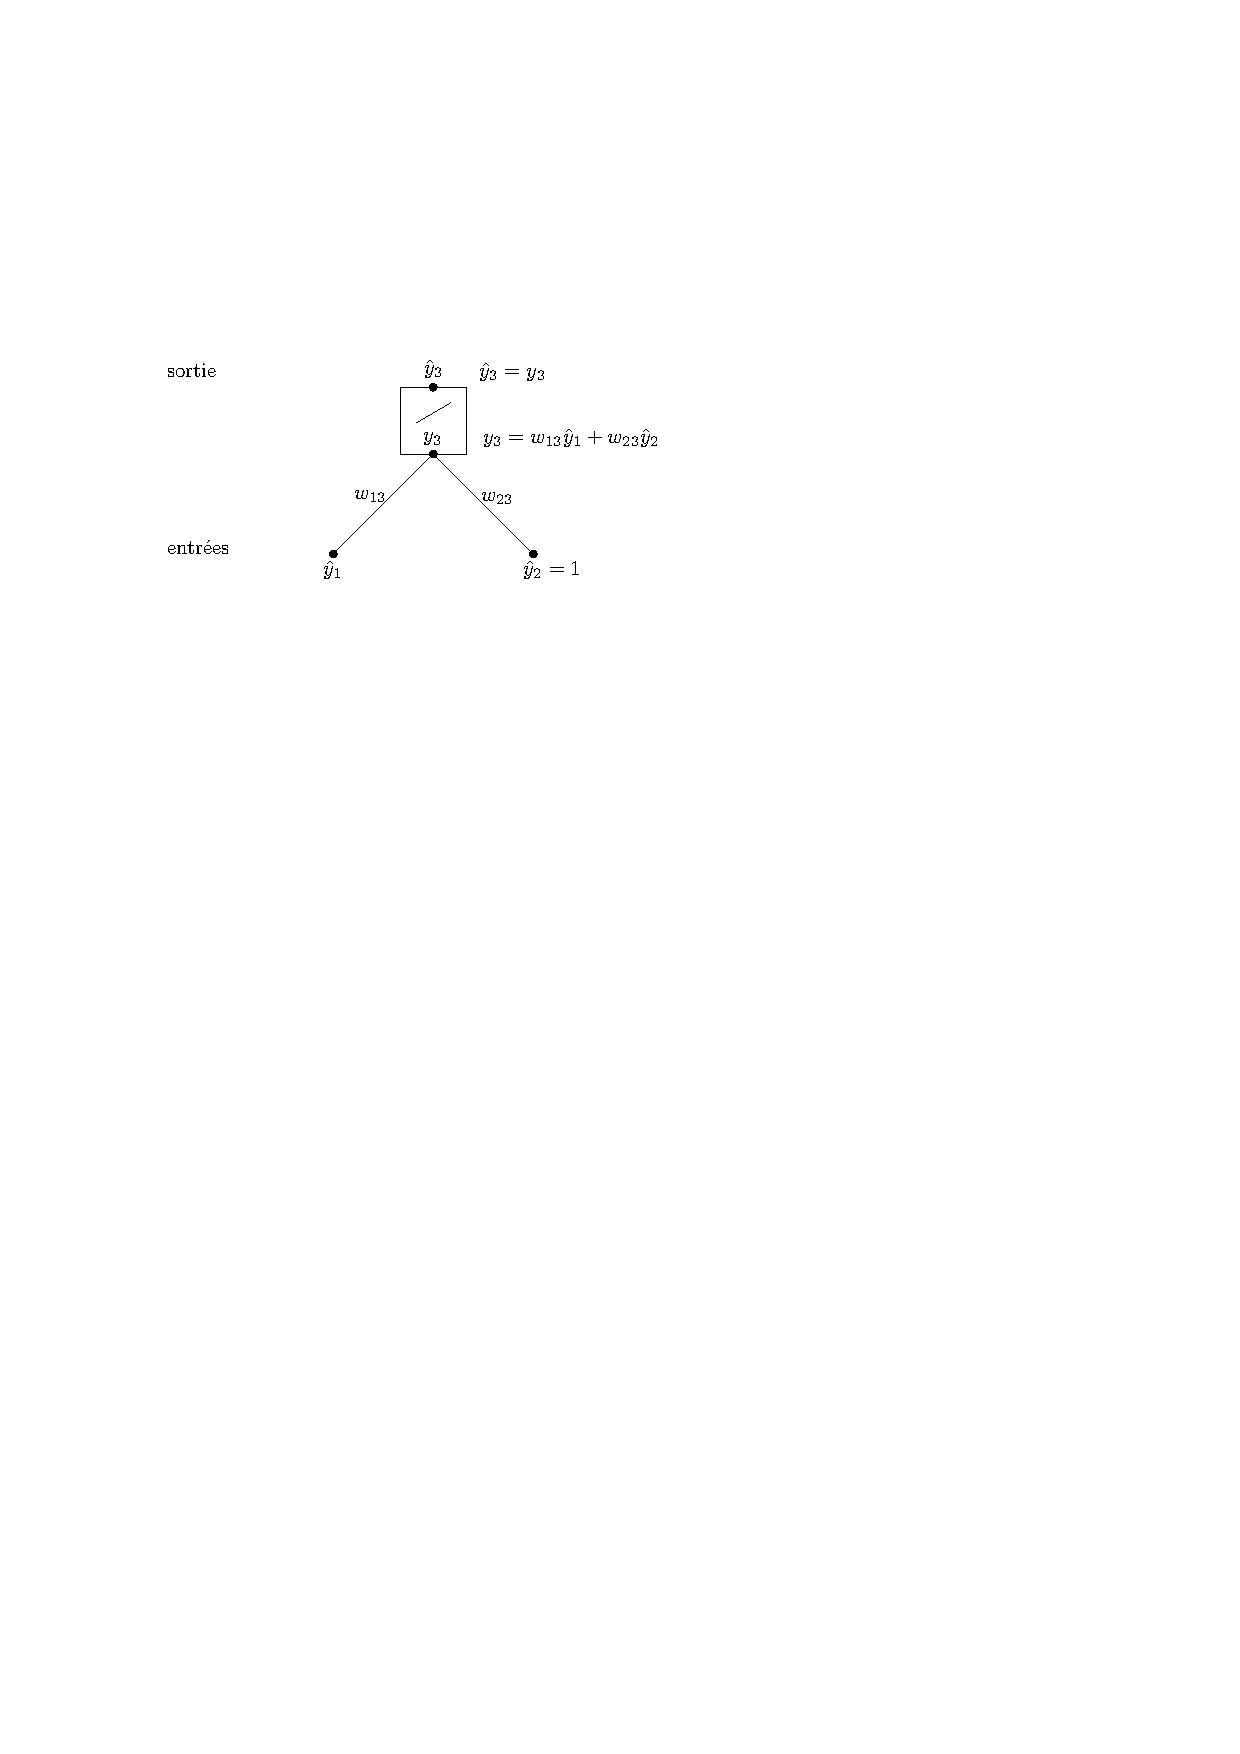
\includegraphics[width=0.7\textwidth]{rn.pdf}
    \caption{Modélisation de la méthode des moindre carrés par un réseau de neurones.
      En reprenant les notations de la section~\ref{sec:mc}, à chaque fois qu'on nourrit
      le réseau avec la valeur $\hat{y}_1 = u_i$, le réseau retourne la prédiction $\hat{y}_3 = \hat{v}_i$,
      calculée à partir des valeurs $x_1 = w_{13}$ et $x_2 = w_{23}$. }
    \label{fig:rn}
  \end{figure}
  
\end{solution}

\begin{exercice}
Quel est le problème d'optimisation posé ?
Quelle méthode d'optimisation est employée pour le résoudre ?
\end{exercice}

\begin{solution}
  L'objectif de l'apprentissage est de trouver le poids des connections assurant que
  pour chaque vecteur d'entrées, le vecteur de sorties du réseau est suffisamment proche
  de la sortie attendue. Pour un ensemble d'observation entrées-sorties, il s'agit de
  trouver la pondération qui minimise le carré des écarts entre les sorties observées
  pour des entrées données et les sorties prédites par le réseau pour les mêmes entrées
  (cf. équation 3 de \cite{hinton86}).

  La méthode d'optimisation proposée est une méthode itérative de descente de gradient
  (cf. équations 8 et 9 de \cite{hinton86}), le gradient étant lui-même calculé par
  rétro-propagation (cf. équations 4 à 7 de \cite{hinton86}).
\end{solution}

\bibliographystyle{plain}
\bibliography{refs}

\end{document}


